\documentclass[french]{beamer}

\usepackage[utf8]{inputenc}
\usepackage[T1]{fontenc}
\usepackage{lmodern}
\usepackage{babel}
\usepackage{tikz}
\usepackage{graphicx}
\usetikzlibrary{arrows}
\usepackage{caption} 
\captionsetup{position=below}

\usetheme{PaloAlto}

\tikzset{
  treenode/.style = {align=center, inner sep=0pt, text centered,
    font=\sffamily},
  arn_equi/.style = {treenode, circle, white, draw=green, fill=green, text width=1em},
  arn_notequi/.style = {treenode, circle, white, draw=red,fill=red, text width=1em},
  arn_new/.style = {treenode, circle, white, draw=blue,fill=blue, text width=1em},
  arn_null/.style = {treenode, rectangle, draw=black,minimum width=0.5em, minimum height=0.5em}
}



%Pour le TITLEPAGE
\title{Compression}
\subtitle{Projet Mathématiques et Informatique}
\author[]{LABADENS Lucas, \\ MARINO Isabelle}
\date{13 Juin 2016}
\institute[L3 S6-- Informatique]{Université Paris 7 Diderot}


\begin{document}

\begin{frame}
	\titlepage
\end{frame}

\begin{frame}
	\frametitle{Sommaire}
	\tableofcontents	
\end{frame}

\section{La compression: définition }
\begin{frame}{La Compression}
	\textbf{Plusieurs types de compression} :
	\begin{itemize}
	\item<2-4>  Compression avec perte de données
	\item<3-4>  Compression sans perte de données
	\item <4> Exemples: ZIP, GZIP, XZ, BZIP2,...
	\end{itemize}
\end{frame}

\section{Huffman}
\begin{frame}{Huffman}
	\begin{center}
	\textbf{Caractéristique} :\\
	
	\begin{itemize}
	\item  Un codage entropique
	\item  repose sur la redondance de caractère
	\item code un caractère non plus sur un octet mais sur un nombre de bit 
	\end{itemize}
	\end{center}
\end{frame}

\begin{frame}{Compression}

	\textbf{Étape} :\\
	
\begin{itemize}
	\item compte des redondances de caractères
	\item création de l'arbre de compression en fonction des poids des caractères 
		
	\item récupération des nouveaux codes de chaque caractère
	\item relecture du fichier pour écrire chaque caractère dans le fichier compresser avec son nouveau code
	\item on complète le dernière octet par la convention un 1 puis le nombre de 0 nécessaire
	\end{itemize}

\end{frame}
\begin{frame}{Compression}
	\textbf{Création de l'arbre}	\\
	\begin{itemize}
			\item on crée des feuilles qui sont des poids munie d'un caractère
			\item on relie les deux feuilles de poids de plus faible par un nœud qui est un poids muni d'un fils gauche et droit
			\item on relie les poids les deux poids les plus faibles par un nouveau  jusqu'à ne plus avoir qu'un seul nœud
		\end{itemize}
\end{frame}
\begin{frame}{Décompression}
\textbf{Étape} :\\
\begin{itemize}
\item<1-5> récupération de l'arbre de compression
\item<2-5> lecture du fichier compresser bit à bit et parcours de l'arbre :
	\begin{itemize}
		\item<3-5> lecture d'un 0 on se déplace à gauche et sinon à droite
		\item<4-5> lorsque l'on tombe sur une feuille on écrit son caractère associé dans le fichier de décompression
	\end{itemize}
\item<5> attention à ne pas lire les bits complétant le dernière octet du fichier
\end{itemize}
\end{frame}

\begin{frame}{Exemple}
	\begin{center}
	\textbf{Étape 1} \\
	Soit un texte ou il est écrit :  aaaabcbbce \\
	(a,4) (b,3) (c,2) (e,1)
	\end{center}
\end{frame}
\begin{frame}{Exemple}
	\begin{center}
	\textbf{Étape 2} \\
	\begin{tikzpicture}
	\node (0) at (0,0) {3};
	\node (1) at (-1,-1) {(e,1)};
	\node (2) at (1,-1) {(c,2)};
	\node (3) at (3,-1/2) {(b,3)};
	\node (4) at (5,-1/2) {(a,4)};
	\draw [-,>=latex,](0)--(1) node[pos=0.6,left, above]{0};
	\draw [-,>=latex,](0)--(2) node[pos=0.6,right, above]{1};
	\end{tikzpicture}	
	\end{center}
\end{frame}
\begin{frame}{Exemple}
	\begin{center}

	\textbf{Etape 3} \\

	\begin{tikzpicture}
	\node (0) at (0,0) {3};
	\node (1) at (-1,-1) {(e,1)};
	\node (2) at (1,-1) {(c,2)};
	\node (3) at (2,0) {(b,3)};
	\node (4) at (5,-1/2) {(a,4)};
	\node(5) at 	(1,1){6};
	\draw [-,>=latex,](0)--(1) node[pos=0.6,left, above]{0};
	\draw [-,>=latex,](0)--(2) node[pos=0.6,right, above]{1};
	\draw [-,>=latex,](5)--(0) node[pos=0.6,left, above]{0};
	\draw [-,>=latex,](5)--(3) node[pos=0.6,right, above]{1};
	\end{tikzpicture}	
	\end{center}
\end{frame}
\begin{frame}{Exemple}
	\begin{center}
	\textbf{Etape 4} \\

	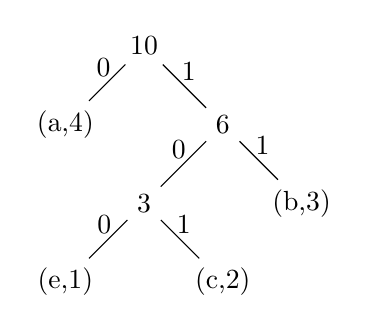
\begin{tikzpicture}
	\node (0) at (0,0) {3};
	\node (1) at (-1,-1) {(e,1)};
	\node (2) at (1,-1) {(c,2)};
	\node (3) at (2,0) {(b,3)};
	\node (4) at (-1,1) {(a,4)};
	\node(5) at 	(1,1){6};
	\node(6) at (0,2){10};
	\draw [-,>=latex,](0)--(1) node[pos=0.6,left, above]{0};
	\draw [-,>=latex,](0)--(2) node[pos=0.6,right, above]{1};
	\draw [-,>=latex,](5)--(0) node[pos=0.6,left, above]{0};
	\draw [-,>=latex,](5)--(3) node[pos=0.6,right, above]{1};
	\draw [-,>=latex,](6)--(4) node[pos=0.6,left, above]{0};
	\draw [-,>=latex,](6)--(5) node[pos=0.6,right, above]{1};
	\end{tikzpicture}	
	\end{center}
\end{frame}
\begin{frame}{Exemple}
\begin{center}

\textbf{Ecriture compresser}\\
les nouveaux codes sont a='0' b='11' c='101' e='100'\\
Le fichier compresser est donc 0 0 0 0 11 101 11 101 100

\end{center}
\end{frame}

\begin{frame}{Exemple: Démonstration}
	\begin{center}
	\textbf{Démonstration}
	\end{center}
\end{frame}

\begin{frame}{Performances}
	\begin{center}
	\begin{tabular}{l | l}
	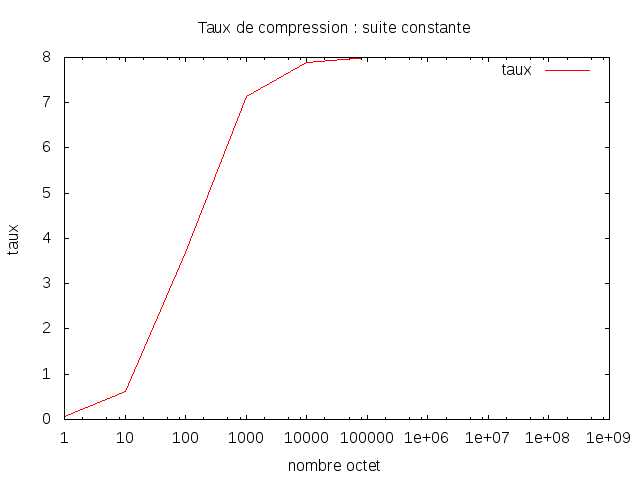
\includegraphics[width=5cm]{HConstant.png} & 
	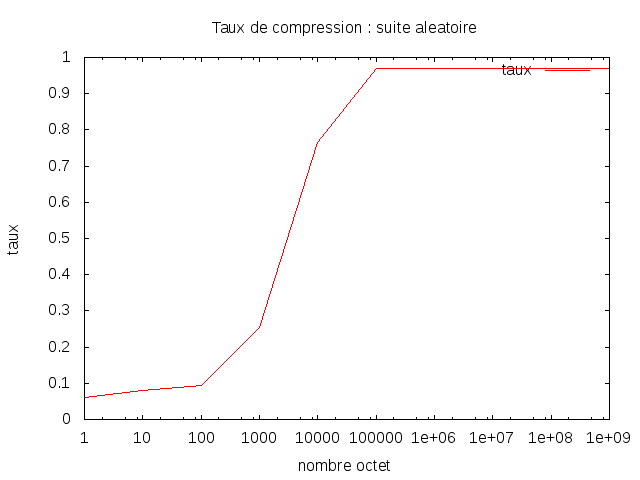
\includegraphics[width=5cm]{aleaH.png}
	\end{tabular}
	\end{center}
\end{frame}

\section{Lempel-Ziv}
\begin{frame}{Lempel-Ziv}
	\begin{center}
	\textbf{Caractéristiques} :
	\begin{itemize}
	\item<2-4>  Codage algorithmique
	\item<3-4>  Bit à bit 
	\item <4>  Code des suites de bits sur le moins de place possible
	\end{itemize}
	\end{center}
\end{frame}


\begin{frame}{Compression}
	\begin{center}
	\textbf{Étape} :
	\begin{itemize}
	\item<2-6>  Création de l'arbre de compression
	\item<3-6>  Étape i : Lecture d'un bit :
			\begin{itemize}
				\item<4-6> 0 : déplacement vers la gauche de l'arbre, lecture du bit suivant
				\item<5-6> 1 : déplacement vers la droite de l'arbre, lecture du bit suivant
				\item<6-6> Déplacement impossible : création de nouveau nœud 
			\end{itemize}
	\end{itemize}
	\end{center}
\end{frame}
	
\begin{frame}{Compression}
	\begin{center}
	\textbf{Étape} :
	\begin{itemize}
	\item<1-2>  Codage et écriture du nouveau nœud dans le fichier
	\item<2> Écriture du bit suivant dans le fichier
	\end{itemize}
	\end{center}
\end{frame}

\begin{frame}{Décompression}
	\begin{center}
	\textbf{Étape} :
		\begin{itemize}
		\item<2-8>  Création d'un tableau à 2 entrées (père, bit)
		\item<3-8> Lecture bit à bit du fichier compressé
		\item<4-8>  A l'étape i : 
			\begin{itemize}
				\item<5-8> Lecture de $\lceil log_{2}(i) \rceil$ (père)
				\item<6-8> Lecture du bit suivant (bit) 
				\item<7-8> Création de la nouvelle case
				\item<8> Écriture de la décompression  
			\end{itemize}
		\end{itemize}
	\end{center}
\end{frame}

\begin{frame}{Exemple : Compression}
	\begin{center}
	Soit un fichier contenant "te"\\
	Suite de bit obtenue : 
	\end{center}	
	\begin{center}	
	01110100 01100101
	\end{center}
\end{frame}

\begin{frame}{Exemple : Compression}
	\begin{center}
	\textbf{Étape 1} \\
	\underline{0} 111010001100101 \\
	\begin{tikzpicture}
	\node (0) at (0,0) {0};
	\node (1) at (-2,-1) {1}; 
	\draw [->,>=latex,](0)--(1) node[pos=0.6,left, above]{0};
	\end{tikzpicture} 
	\end{center}
	\begin{flushleft}
	Écriture dans le fichier : 0
	\end{flushleft}
\end{frame}

\begin{frame}{Exemple : Compression}
	\begin{center}
	\textbf{Étape 2} \\
	\underline{0} \underline{1} 11010001100101 \\
	\begin{tikzpicture}
	\node (0) at (0,0) {0};
\node (1) at (-2,-1) {1}; 
\node (2) at (2,-1) {2};
\draw [->,>=latex,](0)--(1) node[pos=0.6,left, above]{0};
\draw [->,>=latex,](0)--(2) node[pos=0.6,left, above]{1};
	\end{tikzpicture} 
	\end{center}
	\begin{flushleft}
	Écriture dans le fichier : 01
	\end{flushleft}
\end{frame}

\begin{frame}{Exemple : Compression}
	\begin{center}
	\textbf{Étape 3} \\
	\underline{0} \underline{1} \underline{11} 010001100101 \\
	\begin{tikzpicture}
	\node (0) at (0,0) {0};
\node (1) at (-2,-1) {1}; 
\node (2) at (2,-1) {2};
\node(3) at (4, -2) {3};
\draw [->,>=latex,](0)--(1) node[pos=0.6,left, above]{0};
\draw [->,>=latex,](0)--(2) node[pos=0.6,left, above]{1};
\draw [->,>=latex,](2)--(3) node[pos=0.6,left, above]{1};
	\end{tikzpicture} 
	\end{center}
	\begin{flushleft}
	Écriture dans le fichier : 101
	\end{flushleft}
\end{frame}

\begin{frame}{Exemple : Compression}
	\begin{center}
	\textbf{Étape 4} \\
	\underline{0} \underline{1} \underline{11} \underline{01} 0001100101 \\
	\begin{tikzpicture}
	\node (0) at (0,0) {0};
\node (1) at (-2,-1) {1}; 
\node (2) at (2,-1) {2};
\node(3) at (4, -2) {3};
\node(4) at (0, -2) {4};
\draw [->,>=latex,](0)--(1) node[pos=0.6,left, above]{0};
\draw [->,>=latex,](0)--(2) node[pos=0.6,left, above]{1};
\draw [->,>=latex,](2)--(3) node[pos=0.6,left, above]{1};
\draw [->,>=latex,](1)--(4) node[pos=0.6,left, above]{1};
	\end{tikzpicture} 
	\end{center}
	\begin{flushleft}
	Écriture dans le fichier : 011
	\end{flushleft}
\end{frame}

\begin{frame}{Exemple : Compression}
	\begin{center}
	\textbf{Étape 5} \\
	\underline{0} \underline{1} \underline{11} \underline{01} \underline{00} 01100101 \\
	\begin{tikzpicture}
	\node (0) at (0,0) {0};
\node (1) at (-2,-1) {1}; 
\node (2) at (2,-1) {2};
\node(3) at (4, -2) {3};
\node(4) at (0, -2) {4};
\node(5) at (-4, -2) {5};
\draw [->,>=latex,](0)--(1) node[pos=0.6,left, above]{0};
\draw [->,>=latex,](0)--(2) node[pos=0.6,left, above]{1};
\draw [->,>=latex,](2)--(3) node[pos=0.6,left, above]{1};
\draw [->,>=latex,](1)--(4) node[pos=0.6,left, above]{1};
\draw [->,>=latex,](1)--(5) node[pos=0.6,left, above]{0};
	\end{tikzpicture} 
	\end{center}
	\begin{flushleft}
	Écriture dans le fichier : 0010
	\end{flushleft}
\end{frame} 

\begin{frame}{Exemple : Compression}
	\begin{center}
	\textbf{Étape 6} \\
	\underline{0} \underline{1} \underline{11} \underline{01} \underline{00} \underline{011} 00101 \\
	\begin{tikzpicture}
	\node (0) at (0,0) {0};
\node (1) at (-2,-1) {1}; 
\node (2) at (2,-1) {2};
\node(3) at (4, -2) {3};
\node(4) at (0, -2) {4};
\node(5) at (-4, -2) {5};
\node(6) at (2, -3) {6};
\draw [->,>=latex,](0)--(1) node[pos=0.6,left, above]{0};
\draw [->,>=latex,](0)--(2) node[pos=0.6,left, above]{1};
\draw [->,>=latex,](2)--(3) node[pos=0.6,left, above]{1};
\draw [->,>=latex,](1)--(4) node[pos=0.6,left, above]{1};
\draw [->,>=latex,](1)--(5) node[pos=0.6,left, above]{0};
\draw [->,>=latex,](4)--(6) node[pos=0.6,left, above]{1};
	\end{tikzpicture} 
	\end{center}
	\begin{flushleft}
	Écriture dans le fichier : 1001
	\end{flushleft}
\end{frame}

\begin{frame}{Exemple : Compression}
	\begin{center}
	\textbf{Étape 7} \\
	\underline{0} \underline{1} \underline{11} \underline{01} \underline{00} \underline{011} \underline{001} 01 \\
	\begin{tikzpicture}
	\node (0) at (0,0) {0};
\node (1) at (-2,-1) {1}; 
\node (2) at (2,-1) {2};
\node(3) at (4, -2) {3};
\node(4) at (0, -2) {4};
\node(5) at (-4, -2) {5};
\node(6) at (2, -3) {6};
\node(7) at (-2, -3) {7};
\draw [->,>=latex,](0)--(1) node[pos=0.6,left, above]{0};
\draw [->,>=latex,](0)--(2) node[pos=0.6,left, above]{1};
\draw [->,>=latex,](2)--(3) node[pos=0.6,left, above]{1};
\draw [->,>=latex,](1)--(4) node[pos=0.6,left, above]{1};
\draw [->,>=latex,](1)--(5) node[pos=0.6,left, above]{0};
\draw [->,>=latex,](4)--(6) node[pos=0.6,left, above]{1};
\draw [->,>=latex,](5)--(7) node[pos=0.6,left, above]{1};
	\end{tikzpicture} 
	\end{center}
	\begin{flushleft}
	Écriture dans le fichier : 1011
	\end{flushleft}
\end{frame}

\begin{frame}{Exemple : Compression}
	\begin{center}
	\textbf{Étape 8} \\
	\underline{0} \underline{1} \underline{11} \underline{01} \underline{00} \underline{011} \underline{001} \underline{01} \\
	\begin{tikzpicture}
	\node (0) at (0,0) {0};
\node (1) at (-2,-1) {1}; 
\node (2) at (2,-1) {2};
\node(3) at (4, -2) {3};
\node(4) at (0, -2) {4};
\node(5) at (-4, -2) {5};
\node(6) at (2, -3) {6};
\node(7) at (-2, -3) {7};
\draw [->,>=latex,](0)--(1) node[pos=0.6,left, above]{0};
\draw [->,>=latex,](0)--(2) node[pos=0.6,left, above]{1};
\draw [->,>=latex,](2)--(3) node[pos=0.6,left, above]{1};
\draw [->,>=latex,](1)--(4) node[pos=0.6,left, above]{1};
\draw [->,>=latex,](1)--(5) node[pos=0.6,left, above]{0};
\draw [->,>=latex,](4)--(6) node[pos=0.6,left, above]{1};
\draw [->,>=latex,](5)--(7) node[pos=0.6,left, above]{1};
	\end{tikzpicture}  
	\end{center}
	\begin{flushleft}
	Écriture dans le fichier : 1001 et 1000000
	\end{flushleft}
\end{frame}


\begin{frame}{Exemple: Décompression}

\begin{center}
\underline{0} 0110101100101001101110011000000
\end{center}

\begin{center}
	\begin{tabular}{|c|c|c|}
	\hline
	nœud & 0 & 1 \\
	\hline
	père & -1 & 0 \\
	\hline
	bit & -1 & 0 \\
	\hline 
	\end{tabular}
	\begin{center}
	Écriture dans le fichier : 0
	\end{center}
	\end{center}
\end{frame}

\begin{frame}{Exemple: Décompression}
\begin{center}
\underline{0} \underline{01} 10101100101001101110011000000
\end{center}

	\begin{center}
	\begin{tabular}{|c|c|c|c|}
	\hline
	nœud & 0 & 1 & 2 \\
	\hline
	père & -1 & 0 & 0 \\
	\hline
	bit & -1 & 0 & 1 \\
	\hline 
	\end{tabular}
 \begin{center}
	Écriture dans le fichier : 1
	\end{center}

	\end{center}
\end{frame}

\begin{frame}{Exemple: Décompression}
\begin{center}
\underline{0} \underline{01} \underline{101} 01100101001101110011000000
\end{center}

	\begin{center}
	\begin{tabular}{|c|c|c|c|c|c|c|c|c|c|}
	\hline
	nœud & 0 & 1 & 2 & 3 \\
	\hline
	père & -1 & 0 & 0 & 2\\
	\hline
	bit & -1 & 0 & 1 & 1 \\
	\hline 
	\end{tabular}
	\end{center}
	\begin{center}
	Écriture dans le fichier :1 1
	\end{center}
\end{frame}

\begin{frame}{Exemple: Décompression}
\begin{center}
\underline{0} \underline{01} \underline{101} \underline{011} 00101001101110011000000
\end{center}

	\begin{center}
	\begin{tabular}{|c|c|c|c|c|c|c|c|c|c|}
	\hline
	nœud & 0 & 1 & 2 & 3 & 4 \\
	\hline
	père & -1 & 0 & 0 & 2 & 1 \\
	\hline
	bit & -1 & 0 & 1 & 1 & 1 \\
	\hline 
	\end{tabular}
	\end{center}
	\begin{center}
	Écriture dans le fichier : 0 1
	\end{center}
\end{frame}

\begin{frame}{Exemple: Décompression}
\begin{center}
\underline{0} \underline{01} \underline{101} \underline{011} \underline{0010} 1001101110011000000
\end{center}

	\begin{center}
	\begin{tabular}{|c|c|c|c|c|c|c|c|c|c|}
	\hline
	nœud & 0 & 1 & 2 & 3 & 4 & 5 \\
	\hline
	père & -1 & 0 & 0 & 2 & 1 & 1  \\
	\hline
	bit & -1 & 0 & 1 & 1 & 1 & 0 \\
	\hline 
	\end{tabular}
	\end{center}
	\begin{center}
	Écriture dans le fichier : 0 0
	\end{center}
\end{frame}

\begin{frame}{Exemple: Décompression}
\begin{center}
\underline{0} \underline{01} \underline{101} \underline{011} \underline{0010} \underline{1001} 101110011000000
\end{center}

	\begin{center}
	\begin{tabular}{|c|c|c|c|c|c|c|c|c|c|}
	\hline
	nœud & 0 & 1 & 2 & 3 & 4 & 5 & 6 \\
	\hline
	père & -1 & 0 & 0 & 2 & 1 & 1 & 4  \\
	\hline
	bit & -1 & 0 & 1 & 1 & 1 & 0 & 1 \\
	\hline 
	\end{tabular}
	\end{center}
	\begin{center}
	Écriture dans le fichier : 01 1
	\end{center}
\end{frame}

\begin{frame}{Exemple: Décompression}
\begin{center}
\underline{0} \underline{01} \underline{101} \underline{011} \underline{0010} \underline{1001} \underline{1011} 10011000000
\end{center}

	\begin{center}
	\begin{tabular}{|c|c|c|c|c|c|c|c|c|c|}
	\hline
	nœud & 0 & 1 & 2 & 3 & 4 & 5 & 6 & 7 \\
	\hline
	père & -1 & 0 & 0 & 2 & 1 & 1 & 4 & 5  \\
	\hline
	bit & -1 & 0 & 1 & 1 & 1 & 0 & 1 & 1 \\
	\hline 
	\end{tabular}
	\end{center}
	\begin{center}
	Écriture dans le fichier :00  1
	\end{center}
\end{frame}

\begin{frame}{Exemple: Décompression}
\begin{center}
\underline{0} \underline{01} \underline{101} \underline{011} \underline{0010} \underline{1001} \underline{1011} \underline{1001} 1000000
\end{center}

\begin{center}
	\begin{tabular}{|c|c|c|c|c|c|c|c|c|c|}
	\hline
	nœud & 0 & 1 & 2 & 3 & 4 & 5 & 6 & 7 & 8 \\
	\hline
	père & -1 & 0 & 0 & 2 & 1 & 1 & \textbf{4} & 5 & \textbf{4} \\
	\hline
	bit & -1 & 0 & 1 & 1 & 1 & 0 & \textbf{1} & 1 & \textbf{1} \\
	\hline 
	\end{tabular}
	\end{center}
	\begin{center}
	Écriture dans le fichier : 01
	\end{center}
\end{frame}


\begin{frame}{Exemple: Démonstration}
	\begin{center}
	\textbf{Démonstration}
	\end{center}
\end{frame}

\begin{frame}{Performances}
	\begin{center}
	\begin{tabular}{l | l}
	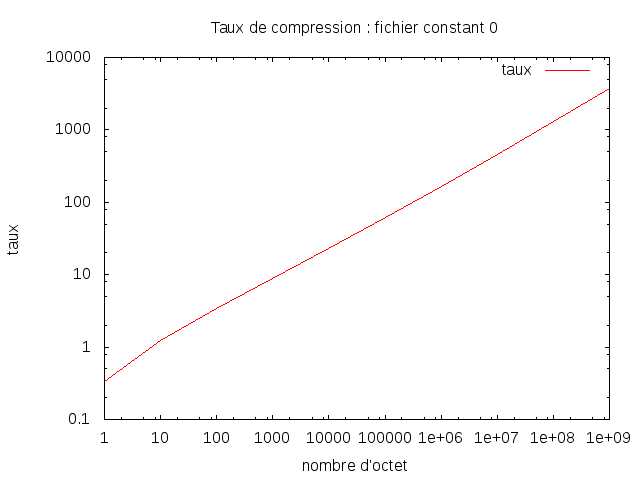
\includegraphics[width=5cm]{LZConstant.png} & 
	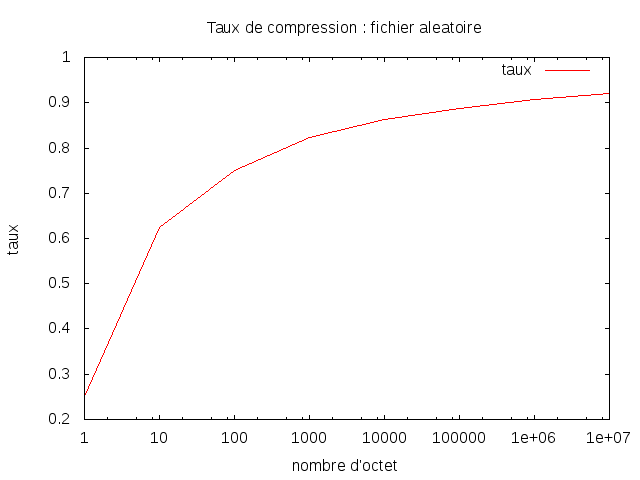
\includegraphics[width=5cm]{LZAleatoire.png}
	\end{tabular}
	\end{center}
\end{frame}



\section{Différences entre les algorithmes}
\begin{frame}{Temps d'exécution à la compression} 
	\begin{center}
	\begin{tabular}{c | c}
	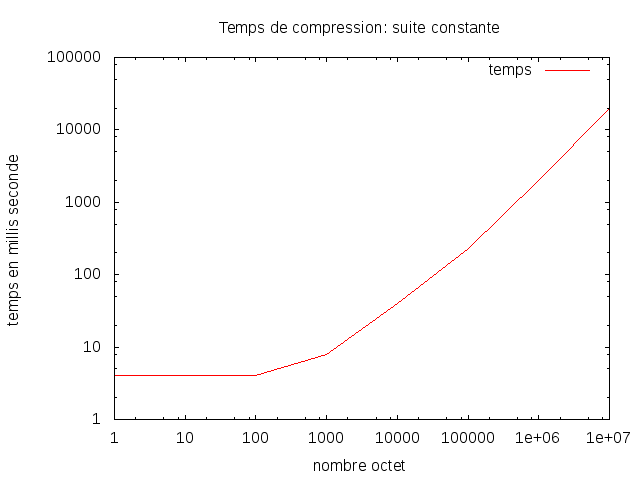
\includegraphics[width=5cm]{tempsChC.png} & 
	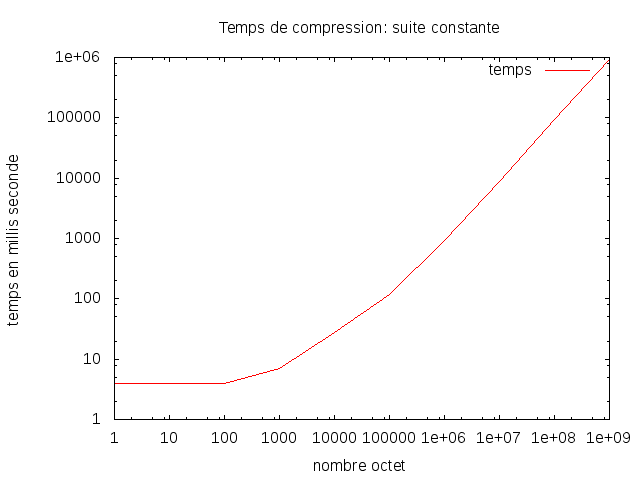
\includegraphics[width=5cm]{tempsClzC.png} \\  &  \\ 
	Huffman & Lempel-Ziv
	\end{tabular}
		\end{center}
\end{frame}
	
\begin{frame}{Temps d'exécution à la compression} 
	\begin{center}
	\begin{tabular}{c | c}
	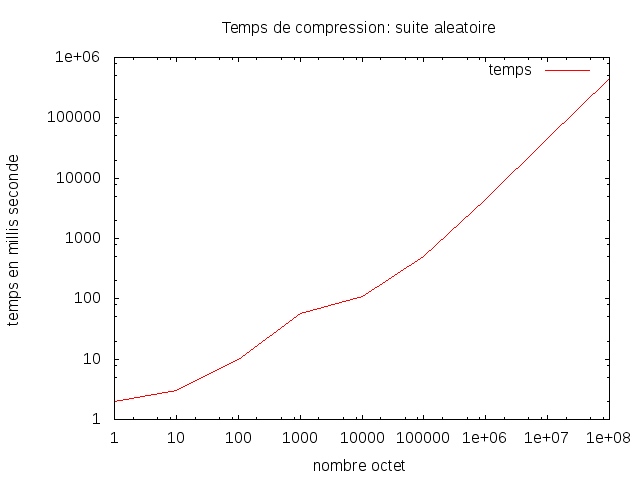
\includegraphics[width=5cm]{tempsChA.png} & 
	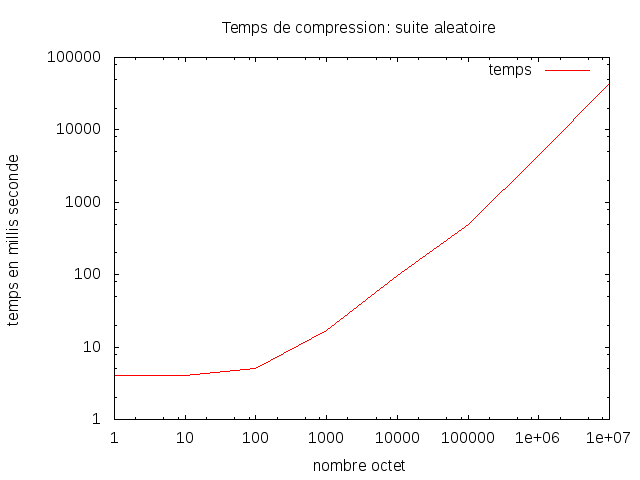
\includegraphics[width=5cm]{tempsClzA.png}
	\\  &  \\ 
	Huffman & Lempel-Ziv
	\end{tabular}	
	\end{center}
\end{frame}

\begin{frame}{Temps d'exécution à la décompression}
	\begin{center}
	\begin{tabular}{c | c}
	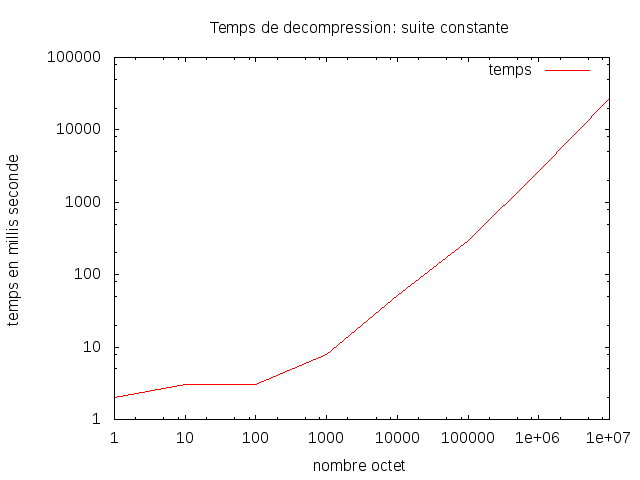
\includegraphics[width=5cm]{tempsDhC.png} & 
	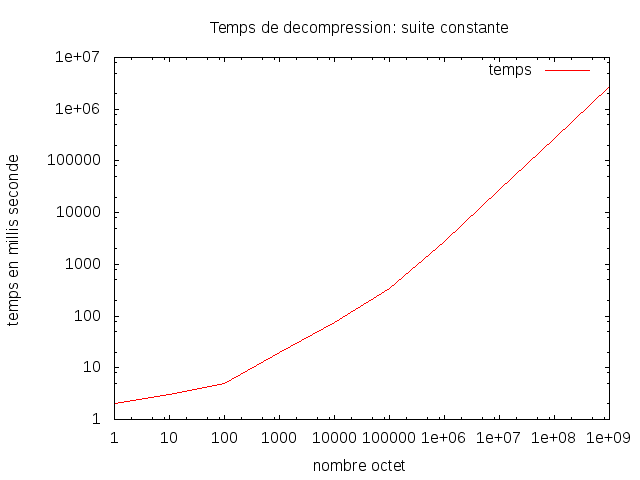
\includegraphics[width=5cm]{tempsDlzC.png}
	\\  &  \\ 
	Huffman & Lempel-Ziv
	\end{tabular}
	\end{center}
\end{frame}

\begin{frame}{Temps d'exécution à la décompression}
	\begin{center}
	
\begin{tabular}{c| c}
	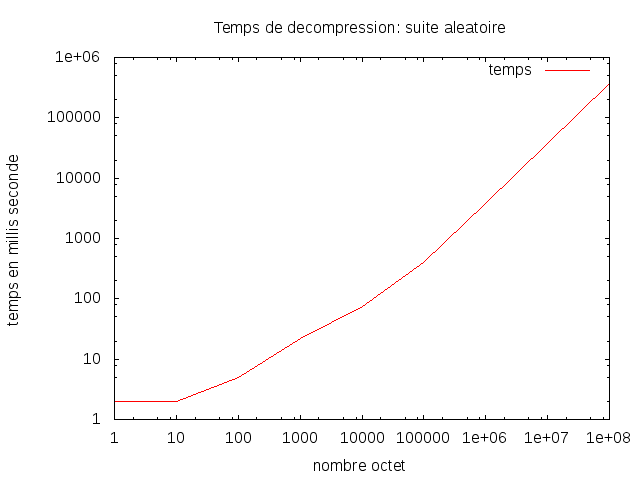
\includegraphics[width=5cm]{tempsDhA.png} & 
	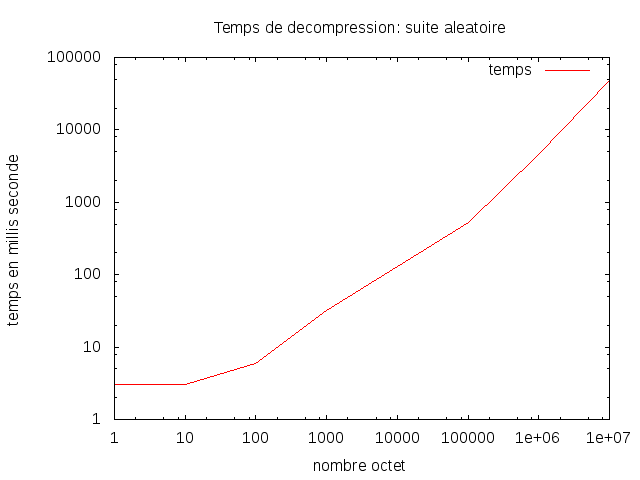
\includegraphics[width=5cm]{tempsDlzA.png}\\  &  \\ 
	Huffman & Lempel-Ziv
	\end{tabular}	
	\end{center}
\end{frame}

\begin{frame}{Différences de structures}
	\begin{center}
	 \begin{itemize}
		\item stockage d'information de compression
		\item nombre de lecture à la compression
		\item base de compression 
		\item limite de taux de compression	
		\item temps d’exécution  
	 
	 \end{itemize}
	\end{center}
\end{frame}

\section{Différences avec les principaux compresseurs}
\begin{frame}{Principales différences}
	\begin{flushleft}
\begin{tabular}{|l|l|l|l|}
\hline
 & La bible & Les Fleurs du Mal  & Au bonheurs \\
 & en anglais & & des Dames \\ 
\hline
taille réelle & 883 158 & 180 199 & 952 753  \\\hline
zip & 3,44 & 2,51 & 2,57  \\
\hline
Gzip & 3,44 & 2,51 & 2,644 \\
\hline
Bzip2 & 4,89 & 3,045 & 3,719 \\
\hline
XZ & 4,649 & 2,826 & 3,323 \\
\hline
Huffman & 1,725 & 1,688 & 1,747  \\
\hline
Lempel-Ziv & 1,796 & 1,310 & 1,482 \\
\hline

\end{tabular}
\end{flushleft}
\end{frame}

\begin{frame}{Principales différences}
	\begin{flushleft}
\begin{tabular}{|l|l|l|l|l|}
\hline
 & fichier & musique & image & vidéo\\
 &  PDF & MP3 & JPG & MOV \\ 
\hline
taille réelle &  198 931 & 8 843 546 & 3 988 442 & 54301053 \\\hline
zip  & 1,246 & 1,065 & 1,002 & 1,0003 \\
\hline
Gzip & 1,247 & 1,065 & 1,002 & 1,0001 \\
\hline
Bzip2 & 1,212 & 1,063 & 1,005 & 0,9961\\
\hline
XZ & 1,261 & 1,066 & 1,002 & 1,0004\\
\hline
Huffman & 0,998 & 1,021 & 0,999 & 0,9999 \\
\hline
Lempel-Ziv & 0,933 & 0,979 & 0,929 & 0,9269\\
\hline

\end{tabular}
\end{flushleft}
\end{frame}

\section{Conclusion}
\begin{frame}{Conclusion}
	\begin{center}
		\begin{itemize}
		\item différence de performance entre Huffman Et Lempel-Ziv
		\item alliance de différent algorithmes plus efficaces
		\item de nouveaux algorithme plus performant à venir
		\end{itemize}
	\end{center}
\end{frame}

\end{document}

